\documentclass{beamer}

\usetheme{Boadilla}

%\includeonlyframes{current}

\usepackage{bookmark}
\usepackage{times}
\usefonttheme{structurebold}
\usepackage{listings}
\usepackage{ragged2e}

\usepackage{pgf}
\usepackage{tikz}
\usepackage{alltt}
\usepackage[normalem]{ulem}
\usetikzlibrary{petri}
\usetikzlibrary{arrows}
\usetikzlibrary{automata}
\usetikzlibrary{shapes}
\usepgflibrary{shapes.geometric}
\usetikzlibrary{shapes.geometric}
\usepackage{amsmath,amssymb}
\usepackage{rotating}
\usepackage{ulem}
\usepackage{listings}
\usepackage{enumerate}
\usepackage{tikz}
\tikzset{
  every overlay node/.style={
    draw=black,fill=white,rounded corners,anchor=north west,
  },
}
\def\tikzoverlay{%
   \tikz[baseline,overlay]\node[every overlay node]
}%

\usepackage{pgfplots}
\usetikzlibrary{automata,arrows}
\tikzstyle{block}=[
   rectangle,
   rounded corners=2mm,
   thick,
   draw=blue!80,
   fill=blue!20,
   align=left,
   minimum size=1cm
]

\tikzstyle{branch}=[
   rectangle,
   rounded corners=2mm,
   thick,
   draw=red!80,
   fill=red!20,
   align=left,
   minimum size=1cm
]

\tikzstyle{merge}=[
   rectangle,
   rounded corners=2mm,
   thick,
   draw=yellow!80,
   fill=yellow!20,
   align=left,
   minimum size=1cm
]

\tikzstyle{try}=[
   rectangle,
   rounded corners=2mm,
   thick,
   draw=violet!80,
   fill=violet!20,
   align=left,
   minimum size=1cm
]

\tikzstyle{catch}=[
   rectangle,
   rounded corners=2mm,
   thick,
   draw=green!80,
   fill=green!20,
   align=left,
   minimum size=1cm
]

\usepackage{listings}
\lstset{
   language=java, 
   basicstyle=\ttfamily,
   columns=fullflexible,
   breaklines=true,
   numbers=left,
   numberstyle=\scriptsize,
   stepnumber=1,
   mathescape=false,
   tabsize=2,
   showstringspaces=false
}
\usepackage{inconsolata}
\newcommand{\predicate}[1] {{\tt \{#1\}}}
%\setbeamercovered{dynamic}
\setbeamertemplate{footline}[page number]{}
\setbeamertemplate{navigation symbols}{}
\usefonttheme{structurebold}

\AtBeginSection{\frame{\sectionpage}}

\defbeamertemplate{section page}{mine}[1][]{%
  \begin{centering}
    {\usebeamerfont{section name}\usebeamercolor[fg]{section name}#1}
    \vskip1em\par
    \begin{beamercolorbox}[sep=12pt,center]{part title}
      \usebeamerfont{section title}\insertsection\par
    \end{beamercolorbox}
  \end{centering}
}

\setbeamertemplate{section page}[mine]

\title{Static and Dynamic Analysis of Test Suites}
\author{Patrick Lam\\University of Waterloo}
\date{October 3, 2015}

\colorlet{redshaded}{red!25!bg}
\colorlet{shaded}{black!25!bg}
\colorlet{shadedshaded}{black!10!bg}
\colorlet{blackshaded}{black!40!bg}

\colorlet{darkred}{red!80!black}
\colorlet{darkblue}{blue!80!black}
\colorlet{darkgreen}{green!80!black}

\newcommand{\rot}[1]{\rotatebox{90}{\mbox{#1}}}
\newcommand{\gray}[1]{\mbox{#1}}
\newenvironment{changemargin}[1]{% 
  \begin{list}{}{% 
    \setlength{\topsep}{0pt}% 
    \setlength{\leftmargin}{#1}% 
    \setlength{\rightmargin}{1em}
    \setlength{\listparindent}{\parindent}% 
    \setlength{\itemindent}{\parindent}% 
    \setlength{\parsep}{\parskip}% 
  }% 
  \item[]}{\end{list}}


\lstset{ %
language=C++,
basicstyle=\ttfamily,commentstyle=\scriptsize\itshape,showstringspaces=false,breaklines=true}

\begin{document}

\begin{frame}
  \titlepage
\end{frame}

\begin{frame}
  \frametitle{Goal}
  \Large
\begin{center}
Convince you to \\ analyze \emph{tests} (with their programs).
\end{center}
\end{frame}


\begin{frame}
  \centering
  \LARGE
  Why do we analyze programs?
\end{frame}

\begin{frame}
  \frametitle{Motivations for Program Analysis}
  \Large
  \begin{changemargin}{1cm}
    \begin{itemize}
    \item enable program understanding \& \\
 \hspace*{2em} transformation;
    \item eliminate bugs;
    \item ensure software quality.
    \end{itemize}
  \end{changemargin}
\end{frame}

% elaborate on these points

\begin{frame}
  \frametitle{Observation}
  \centering
  \LARGE Programs come with gobs of tests.
\end{frame}

\begin{frame}
  \frametitle{Pervasiveness of Test Suites}
\begin{center}
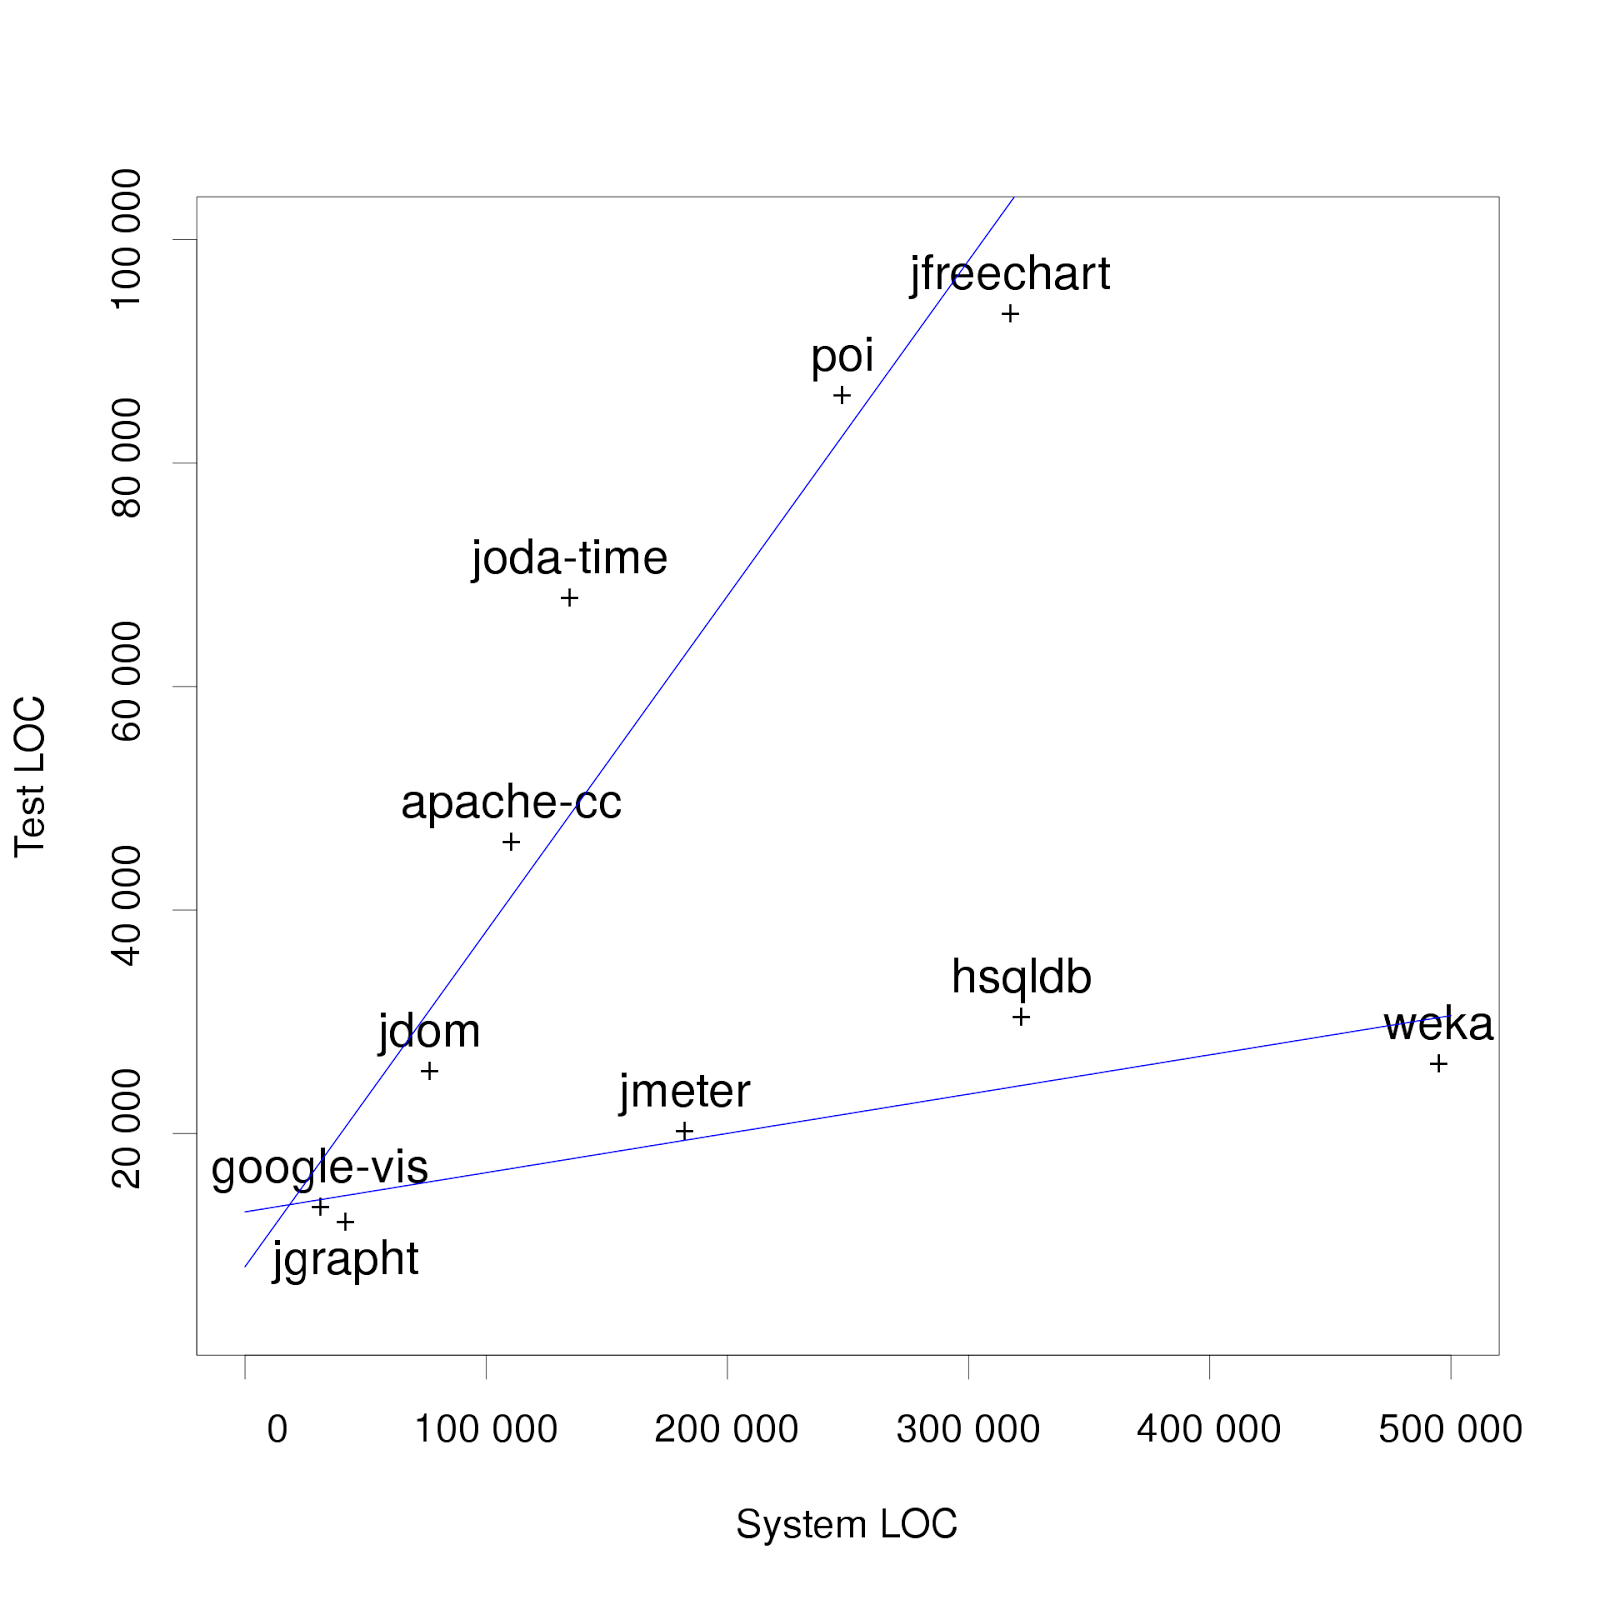
\includegraphics[width=\textwidth, height=.8\textheight, keepaspectratio=true]{images/test-vs-system.png}
\end{center}
\begin{tikzpicture}[remember picture,overlay]
\node [xshift=1cm,yshift=1.3cm] at (current page.center)
{
m=0.3002
};
\node [xshift=1.5cm,yshift=-1.6cm] at (current page.center)
{
m=0.03514
};
\end{tikzpicture}
\end{frame}

\begin{frame}
  \frametitle{Tests and Modern Software}
\Large  Extensive library support:

\begin{center}

\includegraphics[width=.3\textwidth] {images/sunit.png} \\[1em]

\begin{minipage}{.2\textwidth} \vspace*{-2em} 
\includegraphics[width=\textwidth] {images/junit-logo.png} 
\end{minipage}
 \hspace*{3em}

\includegraphics[width=.2\textwidth] {images/Nunit.png}  \hspace*{3em}
\begin{minipage}{.2\textwidth} \vspace*{-1.5em} 
\includegraphics[width=\textwidth] {images/PHPUnit-logo.jpg} 
\end{minipage}
\end{center}

\end{frame}


\begin{frame}
  \frametitle{What Tests Do}

%  A form of lightweight specifications.
%  \begin{itemize}
%  \item executable, provide context
%  \item at various granularities (unit, system)
%  \end{itemize}
\Large 
\begin{changemargin}{1cm}
Tests encode:
\begin{itemize}
\item how to invoke the system under test; and,
\item what it should do.
\end{itemize}
\end{changemargin}

\end{frame}

\begin{frame}
  \frametitle{Opportunity}
\begin{center}
\Large
  Leverage test suites in program analysis.
\end{center}
\end{frame}

\section{Related Work}

\begin{frame}
  \frametitle{Static Analysis Limitations}
\centering

\includegraphics[width=.6\textwidth]{images/soundy.jpg}
\end{frame}

\begin{frame}
  \frametitle{Dynamic Analysis Limitations}

\centering
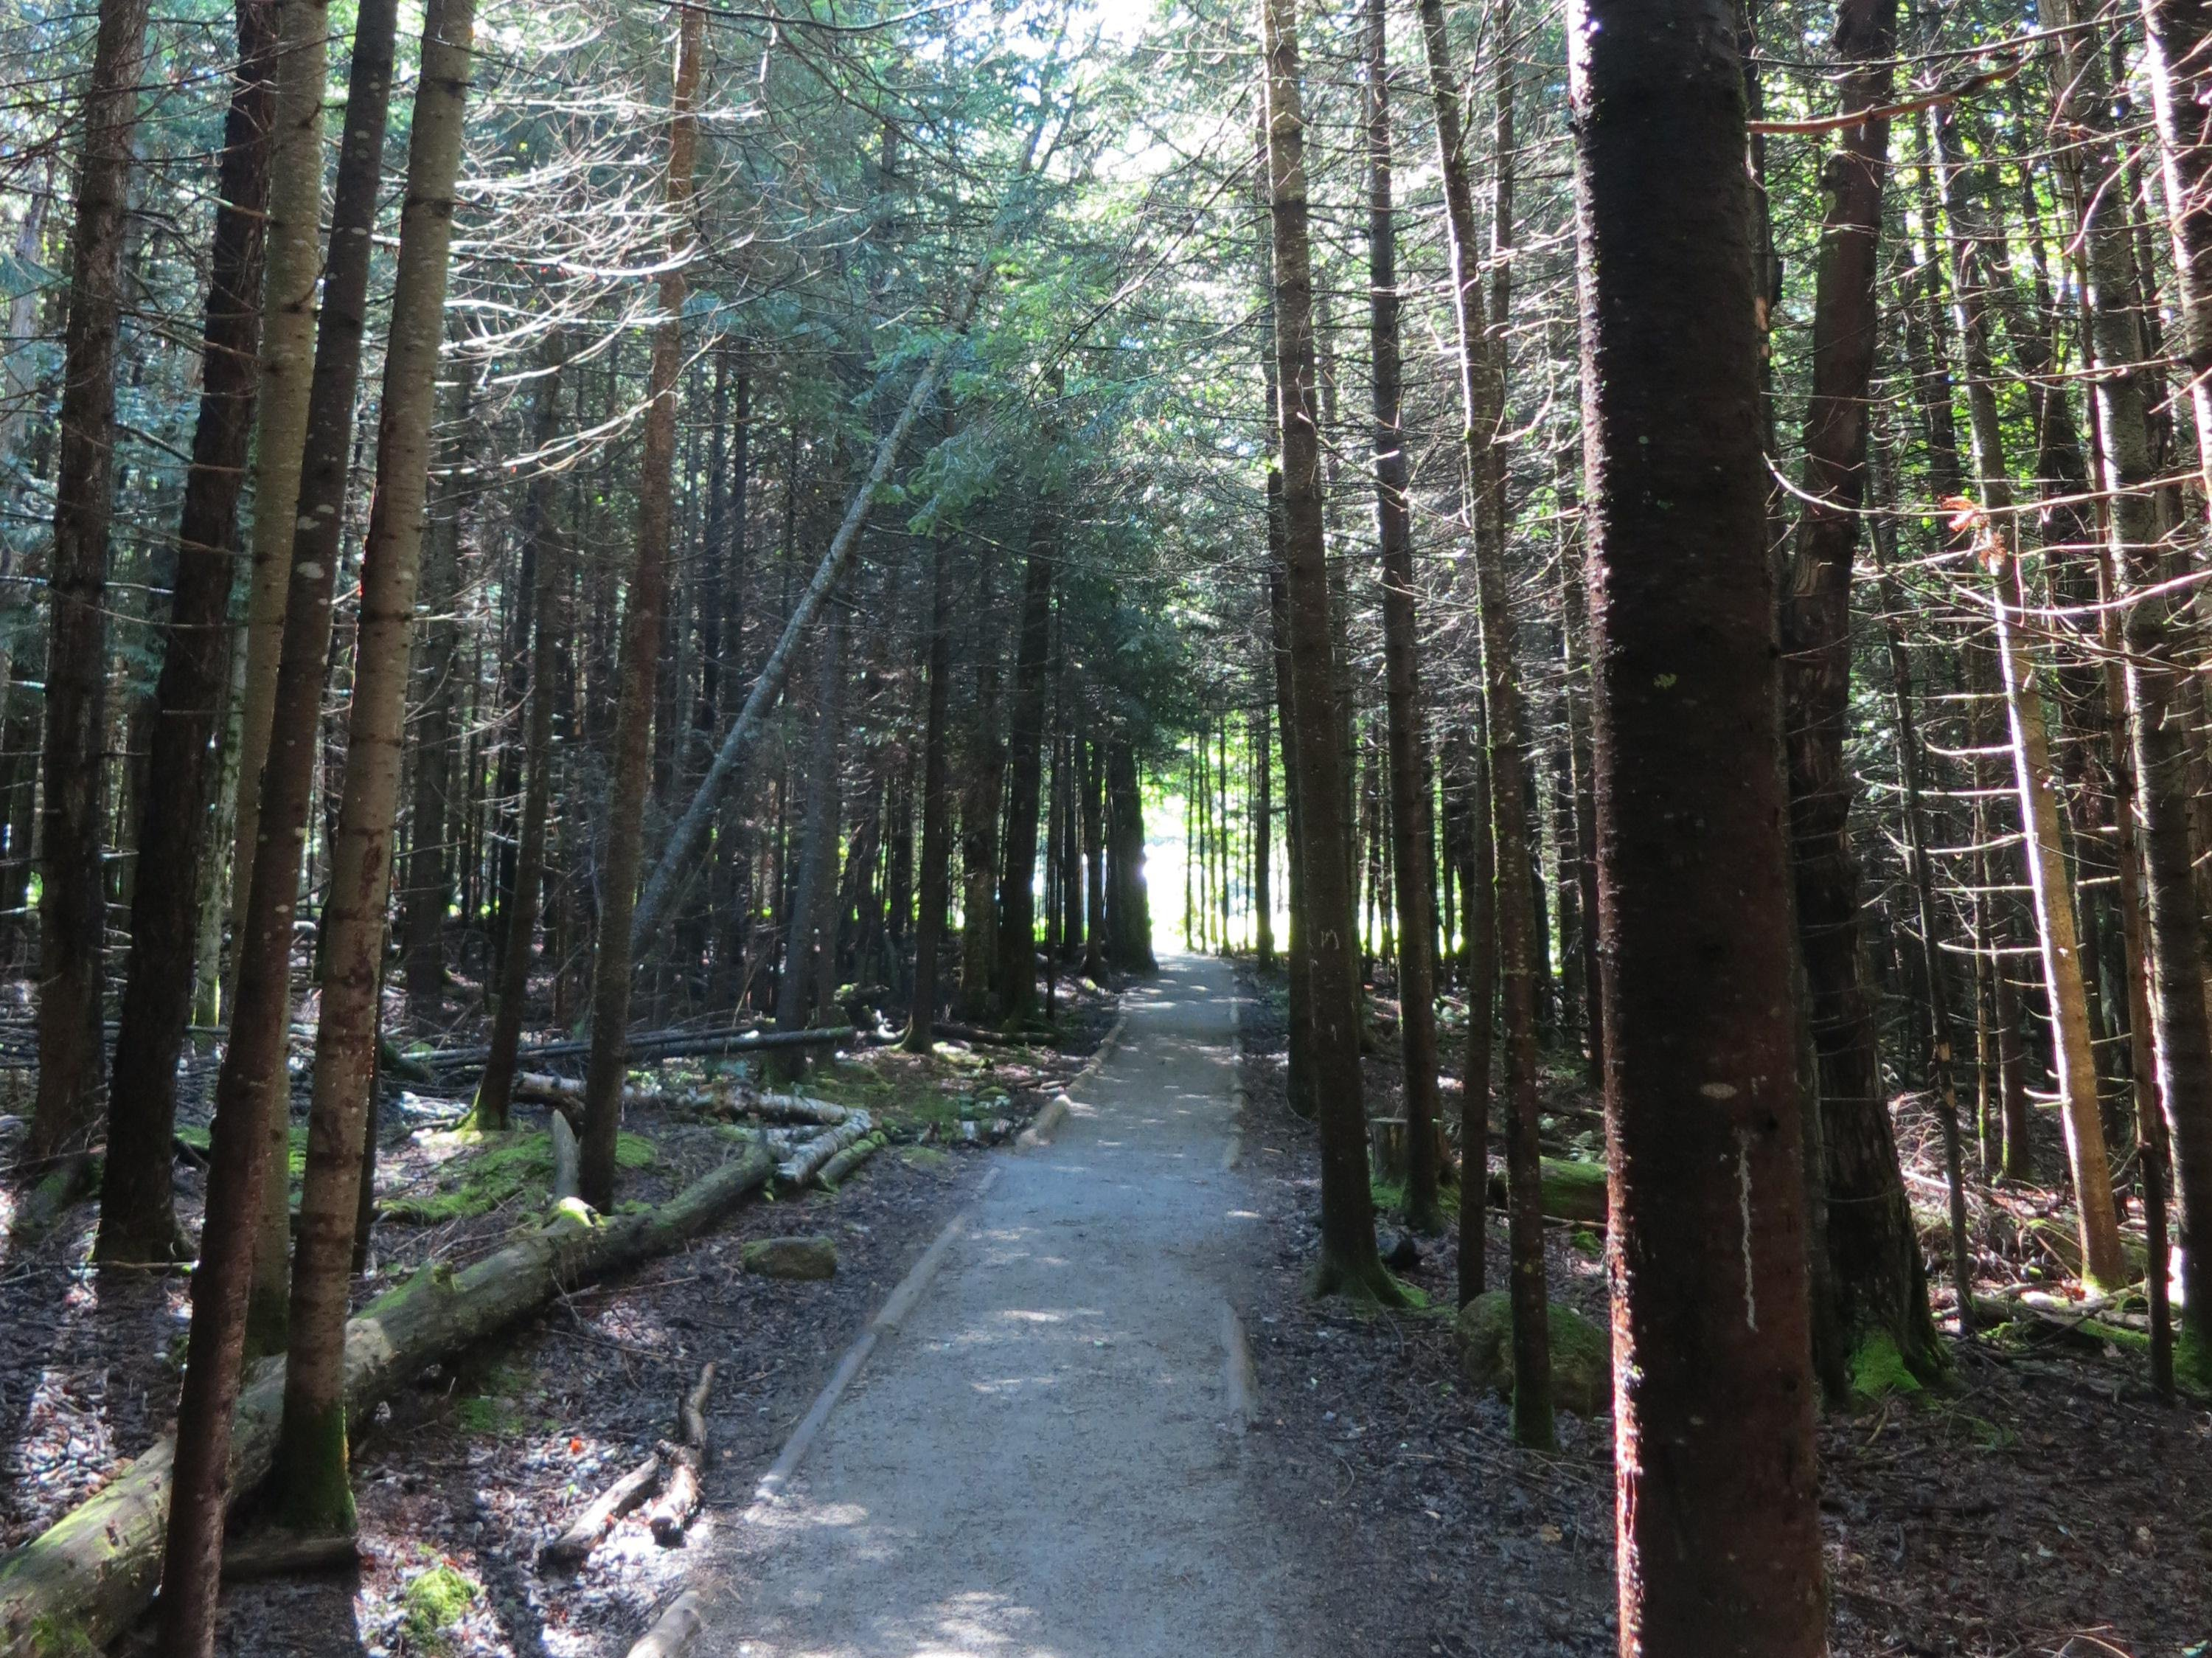
\includegraphics[width=.6\textwidth]{images/0013_class_1_trail.JPG}

\end{frame}


\begin{frame}
  \frametitle{Concolic analysis}

\Large
\begin{changemargin}{1cm}
Run the program with arbitrary inputs, \\
\hspace*{2em} (some symbolic);\\
use solver to find new paths/inputs.
\end{changemargin}
\end{frame}

\begin{frame}
  \frametitle{PHP Analysis (Kneuss, Suter, Kuncak)}

\Large
\begin{center}

\includegraphics[width=.2\textwidth]{images/phantm-blue-solid.png}
\end{center}
\begin{itemize}
\item Choose program inputs and run the program.
\item Observe the configuration loading phase.
\item Use configuration information to do type analysis on the remainder of the program.
\end{itemize}
\end{frame}

\begin{frame}
  \frametitle{TamiFlex (Bodden et al)}

\begin{center}

\includegraphics[width=.2\textwidth]{images/tamiflex.png}
\end{center}

\Large
\begin{changemargin}{1cm}
\begin{itemize}
\item Choose program inputs and run the program.
\item Observe classes loaded through reflection \\
 \hspace*{2em} and custom classloaders.
\end{itemize}
\end{changemargin}

\end{frame}

\begin{frame}
  \frametitle{Dependent Array Type Inference from Tests (Zhu, Nori \& Jagannathan)}

\begin{changemargin}{1cm}
\Large
Goal: learn quantified array invariants.\\[1em]

Approach: observe from test runs; namely:
\begin{itemize}
\item guess coarse templates;
\item run with simple random tests;
\item generate constraints;
\item validate types.
\end{itemize}
\end{changemargin}
\end{frame}

\begin{frame}
  \frametitle{DSD-Crasher (Csallner and Smaragdakis)}

\begin{center}
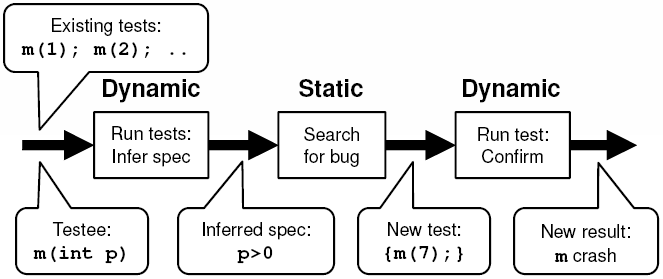
\includegraphics[width=\textwidth]{images/dsd.png}
\end{center}
\end{frame}

\section{Empirical Studies}

\begin{frame}
  \frametitle{Complexity of Test Suites}
\begin{center}
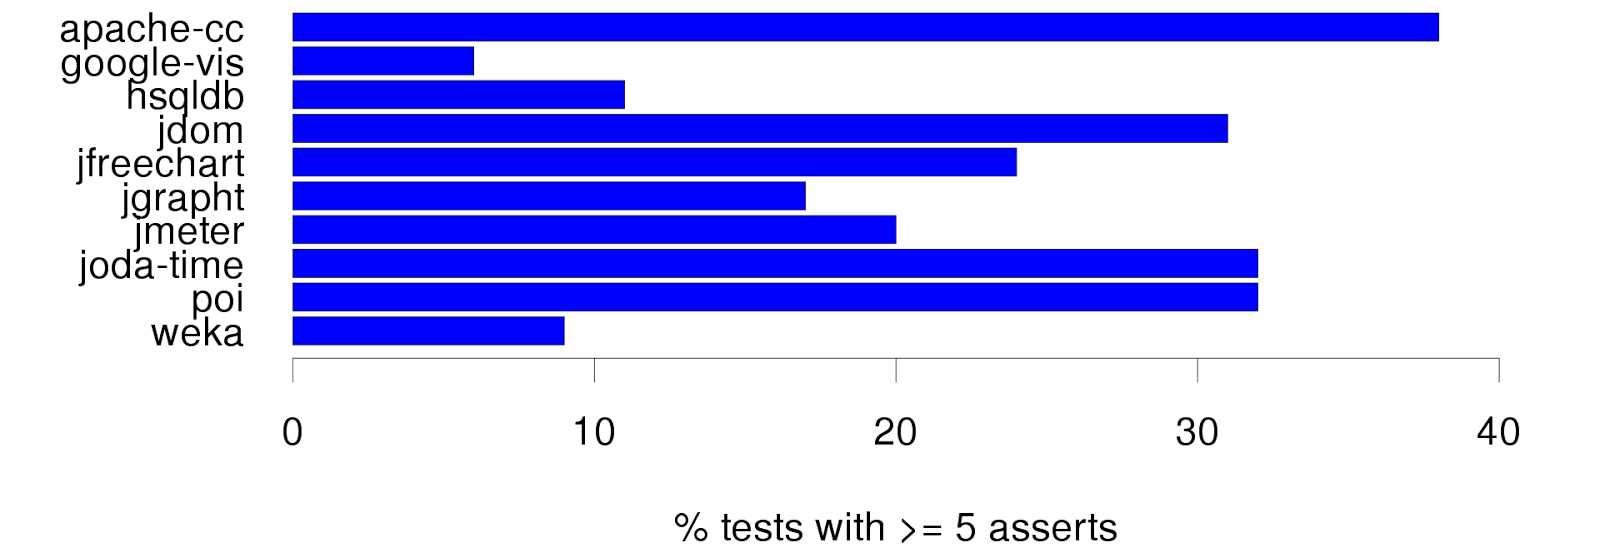
\includegraphics[width=\textwidth, height=.8\textheight, keepaspectratio=true]{images/five-asserts.png}
\end{center}
\end{frame}

\begin{frame}
  \frametitle{\% Tests with control-flow}
\begin{center}
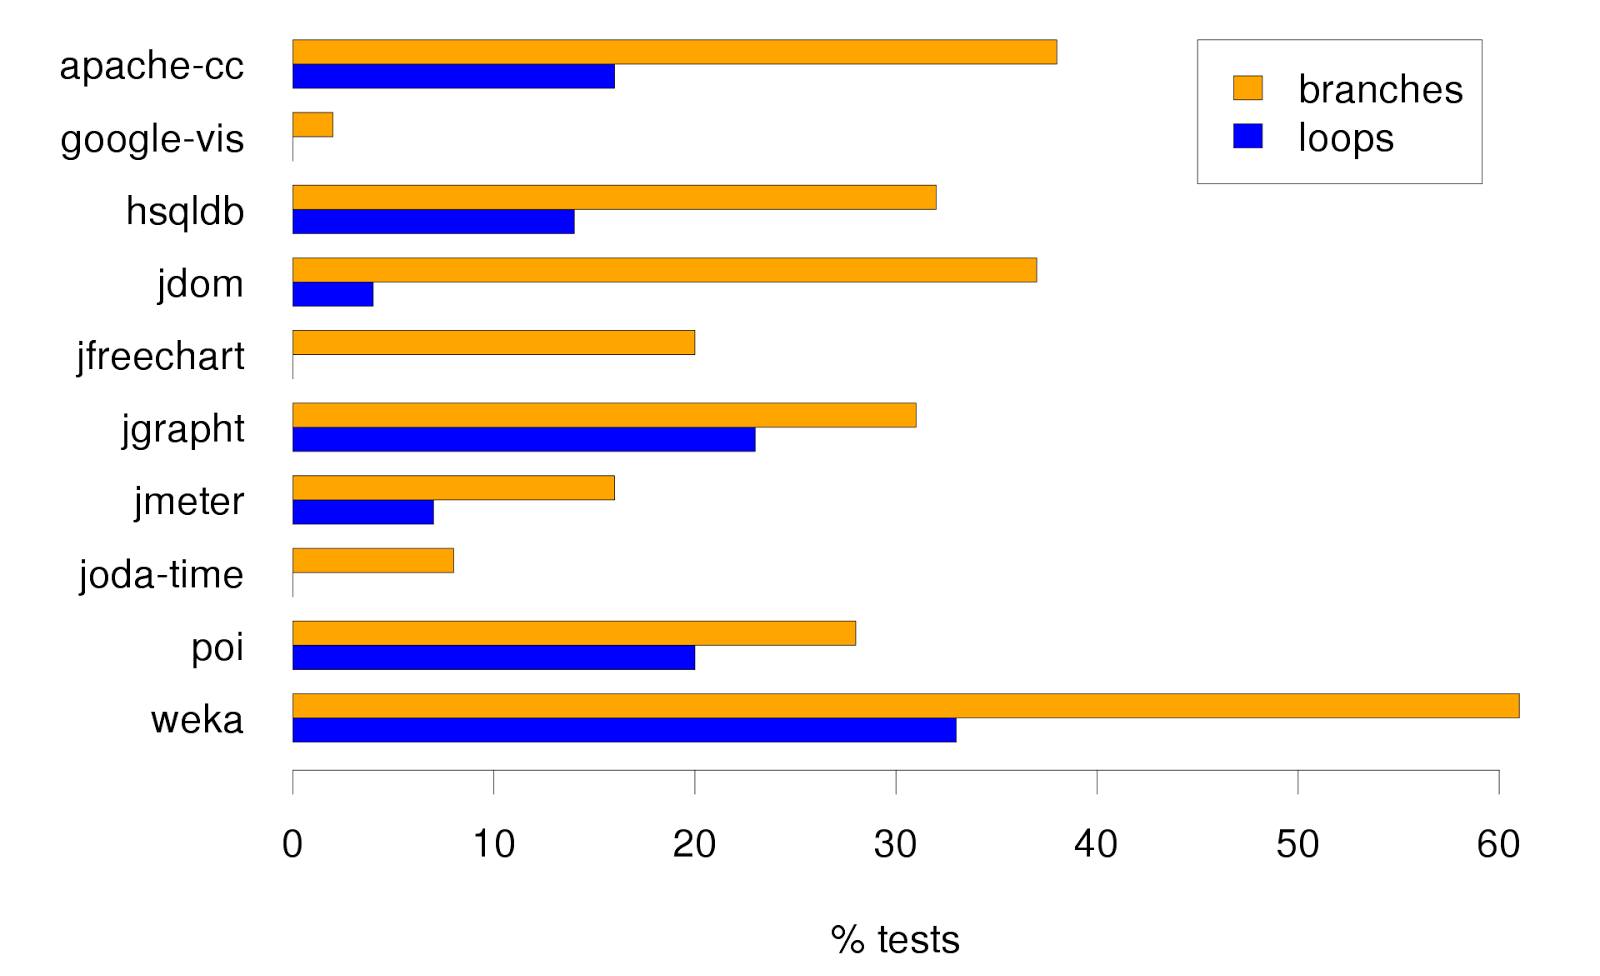
\includegraphics[width=\textwidth, height=.8\textheight, keepaspectratio=true]{images/control-flow.png}
\end{center}
\end{frame}

\begin{frame}
  \begin{centering}
    {\usebeamerfont{section name}\usebeamercolor[fg]{section name}}
    \vskip1em\par
    \begin{beamercolorbox}[sep=12pt,center]{part title}
      \usebeamerfont{section title}Similar Test Methods\\ \small (a case study in static analysis of tests)\par
    \end{beamercolorbox}
\vspace*{2em}
  \end{centering}
\begin{center}
(with Felix Fang)
\end{center}
\end{frame}

\begin{frame}
  \frametitle{Story: Writing Widget class} {\small	
     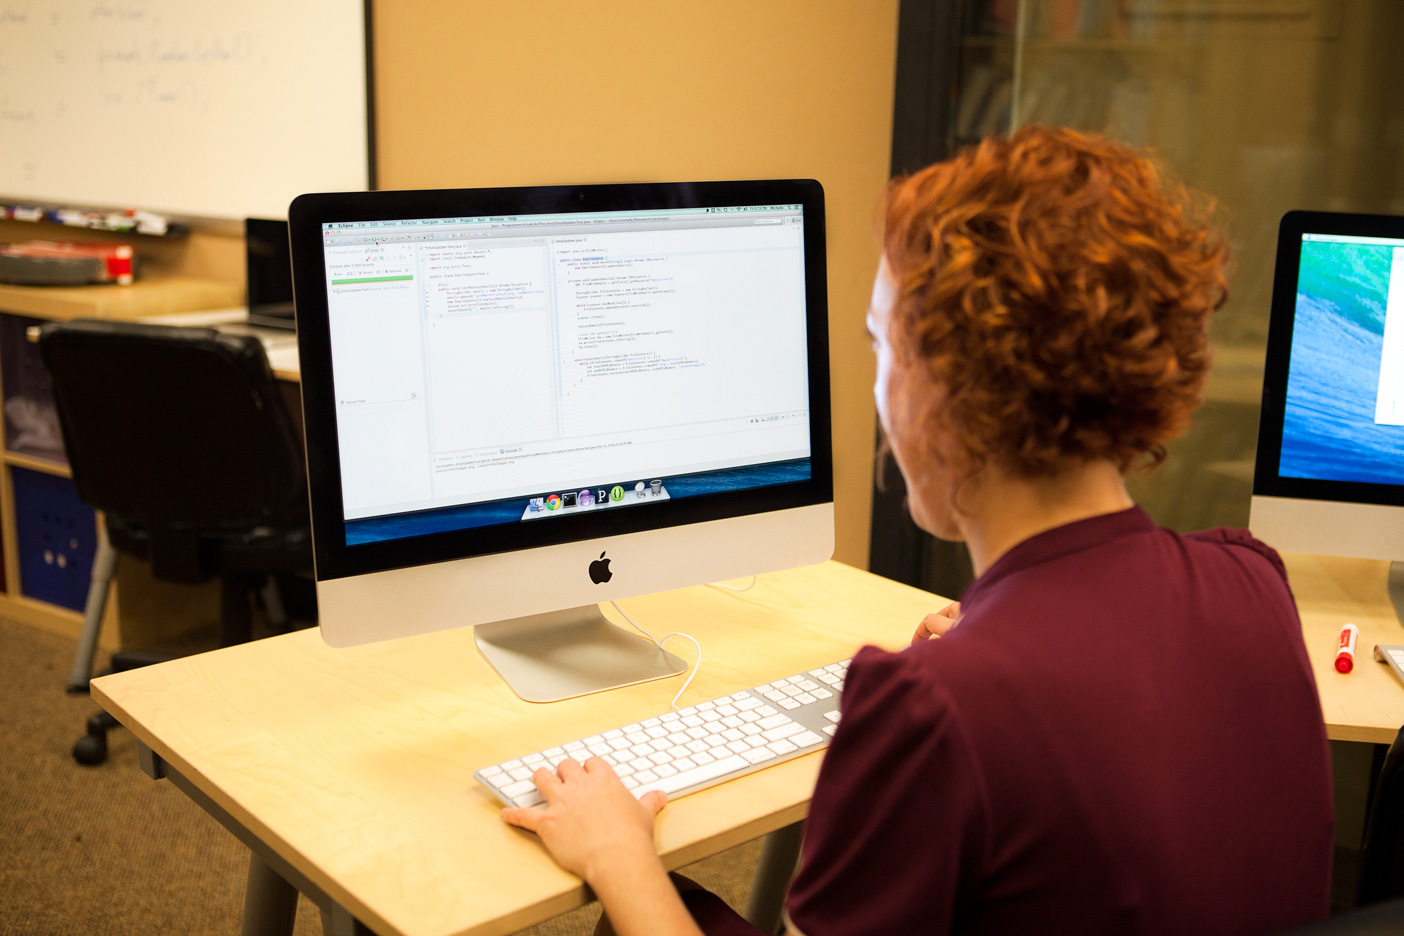
\includegraphics[width=\textwidth, keepaspectratio=true]{images/Programmer_writing_code_with_Unit_Tests.jpg}
     \tiny
     \linebreak
     By Joonspoon (Own work) [CC BY-SA 4.0 (\url{http://creativecommons.org/licenses/by-sa/4.0})], via Wikimedia Commons
  }
\end{frame}

\begin{frame}[fragile]
  \frametitle{Story: Writing Widget class}
  {
     \begin{tabular}{ll}
        \begin{minipage}{0.4\textwidth}
\begin{lstlisting}[]
class FooWidget extends Widget { 
    /*...*/ 
}

class BarWidget extends Widget { 
    /*...*/ 
}
\end{lstlisting}
        \end{minipage}
        &
        \begin{minipage}{0.4\textwidth}
\begin{lstlisting}[]
@Test
class FooWidgetTest { 
    /*...*/ 
}

@Test
class BarWidgetTest { 
    /*...*/ 
}
\end{lstlisting}
        \end{minipage}
     \end{tabular}
  }
\end{frame}

\begin{frame}[fragile]
  \frametitle{Story: Writing New Code}
     \begin{tabular}{ll}
        \begin{minipage}{0.4\textwidth}
\begin{lstlisting}[]
class BazWidget extends Widget { 
    /* New Code */ 
}
\end{lstlisting}
        \end{minipage}
        &
        \begin{minipage}{0.4\textwidth}
\begin{lstlisting}[]
@Test
class BazWidgetTest { 
    /* ? */ 
}
\end{lstlisting}
        \end{minipage}
     \end{tabular}
  
\end{frame}

\begin{frame}[fragile]
  \frametitle{Story: Writing New Code}
     \begin{tabular}{ll}
        \begin{minipage}{0.4\textwidth}
\begin{lstlisting}[]
class BazWidget extends Widget { 
    /* New Code */ 
}
\end{lstlisting}
        \end{minipage}
        &
        \begin{minipage}{0.4\textwidth}
\begin{lstlisting}[]
@Test
class BazWidgetTest { 
/* Ctrl-C, Ctrl-V */ 
}
\end{lstlisting}
        \end{minipage}
     \end{tabular}
\end{frame}

\begin{frame}
  \frametitle{Hypothesis} {\small	
     \vspace*{-1em}
     \Large
     \begin{itemize}
        \item Developers often copy-paste tests \\(and probably enjoy doing it).
           \vspace{0.5cm}
        \item Why? JUnit test cases tend to be self-contained.
           \vspace{1cm}
        \item Test clones can become difficult to comprehend or maintain later.
     \end{itemize}
	}
\end{frame}
\note{
(Show of hands: Who has ever copy-pasted tests before?)
Developers frequently copy-paste tests. It is the easier way to write a bunch of more tests to provide more test coverage. 
Test code is also often overlooked in code review, so those who copy-pasted the tests usually got away with it.
It could have also started with the senior engineers copy-pasting tests, then the others just follow the same bad practice.
(Sometimes I do it too.)

Copy-pasted tests can gradually become extremely difficult to maintain and reduce productivity (if you change the system's behavior, you'd have to update the tests too).

Sometimes there are engineers who would like to help the team out and mitigate the test clone nightmare, but she/he do know where/how to start.

Therefore, the purpose of our research is to help the engineers identify not just test clones, but test refactoring candidates to improve the quality and maintainability of tests.
}

\begin{frame}
  \frametitle{Benefits of Refactoring Tests} {\small	
     \vspace*{-1em}
     \Large
     \begin{itemize}
        \item xUnit Test Patterns: Refactoring Test Code (Meszaros)
           \vspace{0.5cm}
        \item Reduce long term maintenance cost (Saff)
           \vspace{0.5cm}
        \item Can detect new defects and increase branch coverage if tests are parametrized (Thummalapenta et al)
           \vspace{0.5cm}
        \item Reduce brittleness and improve ease of understanding
     \end{itemize}
	}
\end{frame}

\begin{frame}
  \frametitle{Refactoring Techniques} {\small	
     \vspace*{-1em}
     \Large
     \begin{itemize}
        \item Language features such as inheritance or generics
           \vspace{0.5cm}
        \item Parametrized Unit Tests and Theories
     \end{itemize}
	}
\end{frame}
\note{
}

\begin{frame}
  \frametitle{Refactoring Example} {\small	
\begin{changemargin}{.2cm}
     %setID: 37
\begin{lstlisting}
public void testNominalFiltering() {
   m_Filter = getFilter(Attribute.NOMINAL);
   Instances result = useFilter();
   for (int i = 0; i < result.numAttributes(); i++)
      assertTrue(result.attribute(i).type() != Attribute.NOMINAL);
}
\end{lstlisting}
\begin{lstlisting}
public void testStringFiltering() {
   m_Filter = getFilter(Attribute.STRING);
   Instances result = useFilter();
   for (int i = 0; i < result.numAttributes(); i++)
      assertTrue(result.attribute(i).type() != Attribute.STRING);
}
\end{lstlisting}


\end{changemargin}
	}
\end{frame}
\note{
Here is a motivating example. 
The two test methods belong to a refactoring candidate set reported by our analysis. 

By inspection, the two methods are obviously clones, and refactorable as well by parametrizing the methods and using different filtering types. 
There are two more candidates in the set, NUMERIC and DATE, and also refactorable.

This example, however, can be missed by a typical clone detector that uses a token threshold because the number of contiguous identical tokens in this example could possibly be not above the threshold.
}

\begin{frame}
  \frametitle{Refactored Example} {\small	
     \begin{lstlisting}
  static final int [] filteringTypes = {
    Attribute.NOMINAL, Attribute.STRING,
    Attribute.NUMERIC, Attribute.DATE
  };

  public void testFiltering() {
    for (int type : filteringTypes)
      testFiltering(type);
  }

  public void testFiltering(final int type) {
    m_Filter = getFilter(type);
    Instances result = useFilter();
    for (int i = 0; i < result.numAttributes(); i++)
      assertTrue(result.attribute(i).type() != type);
  }
\end{lstlisting}

	}
\end{frame}
\note{
As mentioned previously, this example can be refactored by parametrizing the methods and theorizing data points.
}

\begin{frame}
  \frametitle{Our Contributions} {
     \Large
     \begin{itemize}
        \item Test refactoring candidate detection technique using {\em Assertion Fingerprints}
           \vspace{0.5cm}
        \item Empirical and qualitative analyses of results on 10 Java benchmarks
     \end{itemize}
	}
\end{frame}
\note{
The main contributions of this paper include devising a test refactoring candidate detection technique using Assertion Fingerprints, 
and empirical and qualitative analyses of 10 Java benchmark test suites, of which programs have distinct applications including 
graph theories, machine learning, and data structures.
}

\begin{frame}
  \frametitle{What is a test case made of?} {\small	
     \vspace*{-1em}
     \Large
     \begin{itemize}
        \item Setup
           \vspace{0.5cm}
        \item Run/Exercise
           \vspace{0.5cm}
        \item \alert<2>{Verify}
           \vspace{0.5cm}
        \item Teardown
     \end{itemize}
	}
\end{frame}

\begin{frame}
  \frametitle{Key Insight} {\small	
     \Large
\begin{center}
     Similar tests often have similar sets of asserts.
\end{center}
	}
\end{frame}

\begin{frame}[fragile]
  \frametitle{Similar Sets of Asserts: Example} {\small	
     \begin{tabular}{ll}
        \begin{minipage}{0.51\textwidth}
\begin{lstlisting}[]
public void test1() {
   /* ... */
   assertEqual(int, int);
   /* ... */
   assertEqual(float, float);
   /* ... */
   assertTrue(boolean);
}
\end{lstlisting}
        \end{minipage}
        &
        \begin{minipage}{0.51\textwidth}
\begin{lstlisting}[]
public void test2() {
   /* ... */
   assertEqual(int, int);
   /* ... */
   assertEqual(float, float);
   /* ... */
   assertTrue(boolean);
}
\end{lstlisting}
        \end{minipage}
     \end{tabular}
	}
\end{frame}
\note{}

\begin{frame}
  \frametitle{Our Approach} {\small	
     \hspace*{3em}
     \Huge
     Assertion Fingerprints
	}
\end{frame}

\begin{frame}
  \frametitle{Assertion Fingerprints} {
     \Large
     Augment set of assertions. \\
     \vspace{0.5cm}

     For each assertion call, collect:
     \vspace{0.5cm}

     \begin{itemize}
        \item Parameter types
           \vspace{0.5cm}
        \item {\bf Control flow components}
           \vspace{0.5cm}
     \end{itemize}
	}
\end{frame}

\begin{frame}
  \frametitle{Using Assertion Fingerprints}
\begin{center}
\begin{tikzpicture}[node distance=1.3cm,>=stealth',bend angle=45,auto,
                    every place/.style=     {minimum size=8mm,thick,draw=blue!75,fill=blue!20},
                    every transition/.style={thick,draw=black!75,fill=black!20},
                    red place/.style=       {place,draw=red!75,fill=red!20},
                    blue transition/.style=       {transition,minimum size=8mm,draw=blue!75,fill=blue!20},
                    yellow diamond/.style=       {transition,diamond,minimum size=8mm,draw=yellow!45,fill=yellow!20},
                    every label/.style=     {red}]
      \node[red place, tokens=3] (a) { ~ };
      \node[blue transition, tokens=4, right of=a] (b) { ~ };
      \node[red place, tokens=3, below of=a, xshift=3em] (c) { ~ };
      \node[red place, tokens=3, below of=a, xshift=6em,yshift=1em] (d) { ~ };
      \node[blue transition, tokens=4, below of=a, yshift=-4em] (e) { ~ };
      \node[yellow diamond, tokens=2, below of=a, yshift=-3em, xshift=6em] (e) { ~ };
\end{tikzpicture}
\Large \\
Group tests with similar assert structures.
\end{center}
\end{frame}
\note{
Since assertions form a fundamental part of the structure of JUnit tests, we would like to place a strong focus on them.
We compute Assertion Fingerprints by collecting, for each JUnit assert/fail call, the parameter types, and most importantly, 5 control flow components.
We partition the test methods by the exact same ordered set of assertion fingerprints and report each partition as a clone set.
}

\begin{frame}
  \frametitle{Assertion Fingerprints: Control Flow Components} {
     \Large
     \begin{itemize}
        \item Branch Count (Branch Vertices)
           \vspace{0.5cm}
        \item Merge Count (Merge Vertices)
           \vspace{0.5cm}
        \item In Loop Flag (Depth First Traversal)
           \vspace{0.5cm}
        \item Exceptional Successor Count (Exceptional CFG)
           \vspace{0.5cm}
        \item In Catch Block Flag (Dominator Analysis)
     \end{itemize}
	}
\end{frame}
\note{
The 5 control flow components consider normal control flows such as
branching and loops. We approximate the control flow information
and record number of branch vertices, merge vertices, and boolean flag
of whether the assertion call is in a loop (by depth first traversal)
or not.

We also consider exceptional control flow edges because we discovered
that using try catch blocks in tests is quite common some test suites; 
test suites such as JDOM's include tests that verify if a statement is expected to
throw exceptions and therefore use try catch blocks to construct such
tests. We collect number of exceptional successors for each assertion; 
an exceptional successor count greater than 0 means that the assertion
call is in a try block and have 1 or more number of corresponding
catch blocks.
We also use dominator analysis to detect if an assertion call is in a catch
block.
}

\begin{frame}
  \frametitle{Example: Code} {\small
\begin{changemargin}{.2cm}
     \begin{lstlisting}
public void test() {
   int i;
   for (i = 0; i < 10; ++i) {
      if (i == 2)
         assertEquals(i, 2);
      assertTrue(i != 10);
   }
   try {
      throw new Exception();
      fail("Should have thrown exception");
   } catch (final Exception e) {
      assertEquals(i, 10);
   }
}
\end{lstlisting}

\end{changemargin}
	}
\end{frame}
\note{
Here is a contrived but comprehensive example that covers all 5
control flow components. 
By inspection, one can see that the first two
assertion calls are in a loop, whereas the last two are not.
Also, the fail call obviously is in a try block and has 1 exceptional
successor; the last assertion call is in a catch block. It is
difficult to measure what the branch and merge counts are.
Therefore, the next slide is the control flow graph of this example.
}

\begin{frame}
  \frametitle{Example: CFG} 
\begin{center}
\scalebox{0.8}{
        \begin{tikzpicture}[
         >=latex, 
         node distance=2cm
      ]
      \tiny

      \node (0) [initial, branch] {
         {\tt /*}
         \\{\tt * line 3}
         \\{\tt */}
         \\\predicate{i < 10}
      }; 
      \node (1) [branch, right of=0, xshift=1.8cm] {
         {\tt /*}
         \\{\tt * line 4}
         \\{\tt * bc:1 (\predicate{i<10})}
         \\{\tt * inLoop:true}
         \\{\tt */}
         \\\predicate{i == 2}
      }; 
      \node (2) [try, below of=0, yshift=-1cm] {
         {\tt try:}
         \\{\tt /*}
         \\{\tt * line 10}
         \\{\tt * bc:1 ($\neg$\predicate{i<10})}
         \\{\tt * es:1}
         \\{\tt */}
         \\{\tt fail(String)}
      }; 

      \node (3) [block, below of=1] {
         {\tt /*}
         \\{\tt * line 5}
         \\{\tt * bc:2 (\predicate{i<10},\predicate{i==2})}
         \\{\tt * inLoop:true}
         \\{\tt */}
         \\{\tt assertEquals(int, int)}
      }; 
      \node (4) [merge, below of=3, yshift=-.5cm] {
         {\tt /*}
         \\{\tt * line 6}
         \\{\tt * bc:1 (\predicate{i<10})}
         \\{\tt * mc:1 (\predicate{i==2})}
         \\{\tt * inLoop:true}
         \\{\tt */}
         \\\predicate{i != 10}
      };

      \node (5) [catch, below of=2, yshift=-1cm] {
         {\tt catch:}
         \\{\tt /*}
         \\{\tt * line 12}
         \\{\tt * bc:1 ($\neg$\predicate{i<10})}
         \\{\tt * inCatch:true}
         \\{\tt */}
         \\{\tt assertEquals(int, int)} }; 

      \node (7) [merge, below of=4, yshift=-1cm] {
         {\tt /*}
         \\{\tt * line 6}
         \\{\tt * bc:1 (\predicate{i<10})}
         \\{\tt * mc:2 (\predicate{i==2},\predicate{i!=10})}
         \\{\tt * inLoop:true}
         \\{\tt */}
         \\{\tt assertTrue(boolean)}
      };

      \node (6) [accepting, block, below of=5, yshift=-.3cm] {}; 

      \path[->]

      (0) edge[thick] node [above] {true} (1)
          edge[thick] node [right] {false} (2)

      (1) edge[thick] node [left] {true} (3)
          edge[thick, bend left=47] node [right] {false} (4)

      (2) edge[thick, dashed] node [right] {Exception} (5)
          edge[thick, bend right=47] (6)

      (3) edge[thick] (4)

      (4) edge[thick, bend right=10] node [left] {true} (7)
          edge[thick, bend left=10] node [right] {false} (7)

      (7) edge[thick, out=130, in=320] (0)

      (5) edge[thick] (6)
      ;

   \end{tikzpicture}

}
\end{center}
\end{frame}

\begin{frame}
   \frametitle{Branch Count: Intuition} {\Large	
     \begin{itemize}
        \item An assertion inside an if statement is likely to be different from one that is not.
     \end{itemize}
	}
\end{frame}

\begin{frame}
  \frametitle{Example: CFG} {
\begin{center}
\scalebox{0.8}{
        \begin{tikzpicture}[
         >=latex, 
         node distance=2cm
      ]
      \tiny

      \node (0) [initial, branch] {
         {\tt /*}
         \\{\tt * line 3}
         \\{\tt */}
         \\\predicate{i < 10}
      }; 
      \node (1) [branch, right of=0, xshift=1.8cm] {
         {\tt /*}
         \\{\tt * line 4}
         \\{\tt * bc:1 (\predicate{i<10})}
         \\{\tt * inLoop:true}
         \\{\tt */}
         \\\predicate{i == 2}
      }; 
      \node (2) [try, below of=0, yshift=-1cm] {
         {\tt try:}
         \\{\tt /*}
         \\{\tt * line 10}
         \\{\tt * bc:1 ($\neg$\predicate{i<10})}
         \\{\tt * es:1}
         \\{\tt */}
         \\{\tt fail(String)}
      }; 

      \node (3) [block, below of=1] {
         {\tt /*}
         \\{\tt * line 5}
         \\{\tt * bc:2 (\predicate{i<10},\predicate{i==2})}
         \\{\tt * inLoop:true}
         \\{\tt */}
         \\{\tt assertEquals(int, int)}
      }; 
      \node (4) [merge, below of=3, yshift=-.5cm] {
         {\tt /*}
         \\{\tt * line 6}
         \\{\tt * bc:1 (\predicate{i<10})}
         \\{\tt * mc:1 (\predicate{i==2})}
         \\{\tt * inLoop:true}
         \\{\tt */}
         \\\predicate{i != 10}
      };

      \node (5) [catch, below of=2, yshift=-1cm] {
         {\tt catch:}
         \\{\tt /*}
         \\{\tt * line 12}
         \\{\tt * bc:1 ($\neg$\predicate{i<10})}
         \\{\tt * inCatch:true}
         \\{\tt */}
         \\{\tt assertEquals(int, int)} }; 

      \node (7) [merge, below of=4, yshift=-1cm] {
         {\tt /*}
         \\{\tt * line 6}
         \\{\tt * bc:1 (\predicate{i<10})}
         \\{\tt * mc:2 (\predicate{i==2},\predicate{i!=10})}
         \\{\tt * inLoop:true}
         \\{\tt */}
         \\{\tt assertTrue(boolean)}
      };

      \node (6) [accepting, block, below of=5, yshift=-.3cm] {}; 

      \path[->]

      (0) edge[thick] node [above] {true} (1)
          edge[thick] node [right] {false} (2)

      (1) edge[thick] node [left] {true} (3)
          edge[thick, bend left=47] node [right] {false} (4)

      (2) edge[thick, dashed] node [right] {Exception} (5)
          edge[thick, bend right=47] (6)

      (3) edge[thick] (4)

      (4) edge[thick, bend right=10] node [left] {true} (7)
          edge[thick, bend left=10] node [right] {false} (7)

      (7) edge[thick, out=130, in=320] (0)

      (5) edge[thick] (6)
      ;

   \end{tikzpicture}

}
\end{center}
	}
\end{frame}

\begin{frame}
   \frametitle{Branch Count} {\Large	
     \begin{itemize}
        \item Minimal number of branches needed to reach that vertex from the start of a method, excluding {\tt n}.
     \end{itemize}
	}
\end{frame}

\begin{frame}
   \frametitle{Merge Count: Intuition} {\Large	
     \begin{itemize}
        \item An assertion with some prior operations inside an {\tt if} statement is likely to be different from one that is not with any.
     \end{itemize}
	}
\end{frame}

\begin{frame}
  \frametitle{Example: CFG} {
\begin{center}
\scalebox{0.8}{
        \begin{tikzpicture}[
         >=latex, 
         node distance=2cm
      ]
      \tiny

      \node (0) [initial, branch] {
         {\tt /*}
         \\{\tt * line 3}
         \\{\tt */}
         \\\predicate{i < 10}
      }; 
      \node (1) [branch, right of=0, xshift=1.8cm] {
         {\tt /*}
         \\{\tt * line 4}
         \\{\tt * bc:1 (\predicate{i<10})}
         \\{\tt * inLoop:true}
         \\{\tt */}
         \\\predicate{i == 2}
      }; 
      \node (2) [try, below of=0, yshift=-1cm] {
         {\tt try:}
         \\{\tt /*}
         \\{\tt * line 10}
         \\{\tt * bc:1 ($\neg$\predicate{i<10})}
         \\{\tt * es:1}
         \\{\tt */}
         \\{\tt fail(String)}
      }; 

      \node (3) [block, below of=1] {
         {\tt /*}
         \\{\tt * line 5}
         \\{\tt * bc:2 (\predicate{i<10},\predicate{i==2})}
         \\{\tt * inLoop:true}
         \\{\tt */}
         \\{\tt assertEquals(int, int)}
      }; 
      \node (4) [merge, below of=3, yshift=-.5cm] {
         {\tt /*}
         \\{\tt * line 6}
         \\{\tt * bc:1 (\predicate{i<10})}
         \\{\tt * mc:1 (\predicate{i==2})}
         \\{\tt * inLoop:true}
         \\{\tt */}
         \\\predicate{i != 10}
      };

      \node (5) [catch, below of=2, yshift=-1cm] {
         {\tt catch:}
         \\{\tt /*}
         \\{\tt * line 12}
         \\{\tt * bc:1 ($\neg$\predicate{i<10})}
         \\{\tt * inCatch:true}
         \\{\tt */}
         \\{\tt assertEquals(int, int)} }; 

      \node (7) [merge, below of=4, yshift=-1cm] {
         {\tt /*}
         \\{\tt * line 6}
         \\{\tt * bc:1 (\predicate{i<10})}
         \\{\tt * mc:2 (\predicate{i==2},\predicate{i!=10})}
         \\{\tt * inLoop:true}
         \\{\tt */}
         \\{\tt assertTrue(boolean)}
      };

      \node (6) [accepting, block, below of=5, yshift=-.3cm] {}; 

      \path[->]

      (0) edge[thick] node [above] {true} (1)
          edge[thick] node [right] {false} (2)

      (1) edge[thick] node [left] {true} (3)
          edge[thick, bend left=47] node [right] {false} (4)

      (2) edge[thick, dashed] node [right] {Exception} (5)
          edge[thick, bend right=47] (6)

      (3) edge[thick] (4)

      (4) edge[thick, bend right=10] node [left] {true} (7)
          edge[thick, bend left=10] node [right] {false} (7)

      (7) edge[thick, out=130, in=320] (0)

      (5) edge[thick] (6)
      ;

   \end{tikzpicture}

}
\end{center}
	}
\end{frame}

\begin{frame}
   \frametitle{Merge Count} {\Large    
     \begin{itemize}
        \item Minimal number of merge vertices needed to reach vertex {\tt n} from the start of the method, including {\tt n}.
     \end{itemize}
}
 \end{frame}

\begin{frame}
   \frametitle{In-Loop Flag: Intuition} {\Large	
     \begin{itemize}
        \item An assertion inside a loop is likely to be different from one that is not.
     \end{itemize}
	}
\end{frame}

\begin{frame}
  \frametitle{Example: CFG} {
\begin{center}
\scalebox{0.8}{
        \begin{tikzpicture}[
         >=latex, 
         node distance=2cm
      ]
      \tiny

      \node (0) [initial, branch] {
         {\tt /*}
         \\{\tt * line 3}
         \\{\tt */}
         \\\predicate{i < 10}
      }; 
      \node (1) [branch, right of=0, xshift=1.8cm] {
         {\tt /*}
         \\{\tt * line 4}
         \\{\tt * bc:1 (\predicate{i<10})}
         \\{\tt * inLoop:true}
         \\{\tt */}
         \\\predicate{i == 2}
      }; 
      \node (2) [try, below of=0, yshift=-1cm] {
         {\tt try:}
         \\{\tt /*}
         \\{\tt * line 10}
         \\{\tt * bc:1 ($\neg$\predicate{i<10})}
         \\{\tt * es:1}
         \\{\tt */}
         \\{\tt fail(String)}
      }; 

      \node (3) [block, below of=1] {
         {\tt /*}
         \\{\tt * line 5}
         \\{\tt * bc:2 (\predicate{i<10},\predicate{i==2})}
         \\{\tt * inLoop:true}
         \\{\tt */}
         \\{\tt assertEquals(int, int)}
      }; 
      \node (4) [merge, below of=3, yshift=-.5cm] {
         {\tt /*}
         \\{\tt * line 6}
         \\{\tt * bc:1 (\predicate{i<10})}
         \\{\tt * mc:1 (\predicate{i==2})}
         \\{\tt * inLoop:true}
         \\{\tt */}
         \\\predicate{i != 10}
      };

      \node (5) [catch, below of=2, yshift=-1cm] {
         {\tt catch:}
         \\{\tt /*}
         \\{\tt * line 12}
         \\{\tt * bc:1 ($\neg$\predicate{i<10})}
         \\{\tt * inCatch:true}
         \\{\tt */}
         \\{\tt assertEquals(int, int)} }; 

      \node (7) [merge, below of=4, yshift=-1cm] {
         {\tt /*}
         \\{\tt * line 6}
         \\{\tt * bc:1 (\predicate{i<10})}
         \\{\tt * mc:2 (\predicate{i==2},\predicate{i!=10})}
         \\{\tt * inLoop:true}
         \\{\tt */}
         \\{\tt assertTrue(boolean)}
      };

      \node (6) [accepting, block, below of=5, yshift=-.3cm] {}; 

      \path[->]

      (0) edge[thick] node [above] {true} (1)
          edge[thick] node [right] {false} (2)

      (1) edge[thick] node [left] {true} (3)
          edge[thick, bend left=47] node [right] {false} (4)

      (2) edge[thick, dashed] node [right] {Exception} (5)
          edge[thick, bend right=47] (6)

      (3) edge[thick] (4)

      (4) edge[thick, bend right=10] node [left] {true} (7)
          edge[thick, bend left=10] node [right] {false} (7)

      (7) edge[thick, out=130, in=320] (0)

      (5) edge[thick] (6)
      ;

   \end{tikzpicture}

}
\end{center}
	}
\end{frame}

\begin{frame}
   \frametitle{Exceptional Successors Count: Intuition} {\Large	
     \begin{itemize}
        \item An assertion inside a try block with corresponding catch block(s) is likely to be different from one that is not.
     \end{itemize}
	}
\end{frame}

\begin{frame}
  \frametitle{Example: CFG} {
\begin{center}
\scalebox{0.8}{
        \begin{tikzpicture}[
         >=latex, 
         node distance=2cm
      ]
      \tiny

      \node (0) [initial, branch] {
         {\tt /*}
         \\{\tt * line 3}
         \\{\tt */}
         \\\predicate{i < 10}
      }; 
      \node (1) [branch, right of=0, xshift=1.8cm] {
         {\tt /*}
         \\{\tt * line 4}
         \\{\tt * bc:1 (\predicate{i<10})}
         \\{\tt * inLoop:true}
         \\{\tt */}
         \\\predicate{i == 2}
      }; 
      \node (2) [try, below of=0, yshift=-1cm] {
         {\tt try:}
         \\{\tt /*}
         \\{\tt * line 10}
         \\{\tt * bc:1 ($\neg$\predicate{i<10})}
         \\{\tt * es:1}
         \\{\tt */}
         \\{\tt fail(String)}
      }; 

      \node (3) [block, below of=1] {
         {\tt /*}
         \\{\tt * line 5}
         \\{\tt * bc:2 (\predicate{i<10},\predicate{i==2})}
         \\{\tt * inLoop:true}
         \\{\tt */}
         \\{\tt assertEquals(int, int)}
      }; 
      \node (4) [merge, below of=3, yshift=-.5cm] {
         {\tt /*}
         \\{\tt * line 6}
         \\{\tt * bc:1 (\predicate{i<10})}
         \\{\tt * mc:1 (\predicate{i==2})}
         \\{\tt * inLoop:true}
         \\{\tt */}
         \\\predicate{i != 10}
      };

      \node (5) [catch, below of=2, yshift=-1cm] {
         {\tt catch:}
         \\{\tt /*}
         \\{\tt * line 12}
         \\{\tt * bc:1 ($\neg$\predicate{i<10})}
         \\{\tt * inCatch:true}
         \\{\tt */}
         \\{\tt assertEquals(int, int)} }; 

      \node (7) [merge, below of=4, yshift=-1cm] {
         {\tt /*}
         \\{\tt * line 6}
         \\{\tt * bc:1 (\predicate{i<10})}
         \\{\tt * mc:2 (\predicate{i==2},\predicate{i!=10})}
         \\{\tt * inLoop:true}
         \\{\tt */}
         \\{\tt assertTrue(boolean)}
      };

      \node (6) [accepting, block, below of=5, yshift=-.3cm] {}; 

      \path[->]

      (0) edge[thick] node [above] {true} (1)
          edge[thick] node [right] {false} (2)

      (1) edge[thick] node [left] {true} (3)
          edge[thick, bend left=47] node [right] {false} (4)

      (2) edge[thick, dashed] node [right] {Exception} (5)
          edge[thick, bend right=47] (6)

      (3) edge[thick] (4)

      (4) edge[thick, bend right=10] node [left] {true} (7)
          edge[thick, bend left=10] node [right] {false} (7)

      (7) edge[thick, out=130, in=320] (0)

      (5) edge[thick] (6)
      ;

   \end{tikzpicture}

}
\end{center}
	}
\end{frame}

\begin{frame}
   \frametitle{In-Catch-Block Flag: Intuition} {\Large	
     \begin{itemize}
        \item An assertion inside a catch block is likely to be different from one that is not.
     \end{itemize}
	}
\end{frame}

\begin{frame}
  \frametitle{Example: CFG} {
\begin{center}
\scalebox{0.8}{
        \begin{tikzpicture}[
         >=latex, 
         node distance=2cm
      ]
      \tiny

      \node (0) [initial, branch] {
         {\tt /*}
         \\{\tt * line 3}
         \\{\tt */}
         \\\predicate{i < 10}
      }; 
      \node (1) [branch, right of=0, xshift=1.8cm] {
         {\tt /*}
         \\{\tt * line 4}
         \\{\tt * bc:1 (\predicate{i<10})}
         \\{\tt * inLoop:true}
         \\{\tt */}
         \\\predicate{i == 2}
      }; 
      \node (2) [try, below of=0, yshift=-1cm] {
         {\tt try:}
         \\{\tt /*}
         \\{\tt * line 10}
         \\{\tt * bc:1 ($\neg$\predicate{i<10})}
         \\{\tt * es:1}
         \\{\tt */}
         \\{\tt fail(String)}
      }; 

      \node (3) [block, below of=1] {
         {\tt /*}
         \\{\tt * line 5}
         \\{\tt * bc:2 (\predicate{i<10},\predicate{i==2})}
         \\{\tt * inLoop:true}
         \\{\tt */}
         \\{\tt assertEquals(int, int)}
      }; 
      \node (4) [merge, below of=3, yshift=-.5cm] {
         {\tt /*}
         \\{\tt * line 6}
         \\{\tt * bc:1 (\predicate{i<10})}
         \\{\tt * mc:1 (\predicate{i==2})}
         \\{\tt * inLoop:true}
         \\{\tt */}
         \\\predicate{i != 10}
      };

      \node (5) [catch, below of=2, yshift=-1cm] {
         {\tt catch:}
         \\{\tt /*}
         \\{\tt * line 12}
         \\{\tt * bc:1 ($\neg$\predicate{i<10})}
         \\{\tt * inCatch:true}
         \\{\tt */}
         \\{\tt assertEquals(int, int)} }; 

      \node (7) [merge, below of=4, yshift=-1cm] {
         {\tt /*}
         \\{\tt * line 6}
         \\{\tt * bc:1 (\predicate{i<10})}
         \\{\tt * mc:2 (\predicate{i==2},\predicate{i!=10})}
         \\{\tt * inLoop:true}
         \\{\tt */}
         \\{\tt assertTrue(boolean)}
      };

      \node (6) [accepting, block, below of=5, yshift=-.3cm] {}; 

      \path[->]

      (0) edge[thick] node [above] {true} (1)
          edge[thick] node [right] {false} (2)

      (1) edge[thick] node [left] {true} (3)
          edge[thick, bend left=47] node [right] {false} (4)

      (2) edge[thick, dashed] node [right] {Exception} (5)
          edge[thick, bend right=47] (6)

      (3) edge[thick] (4)

      (4) edge[thick, bend right=10] node [left] {true} (7)
          edge[thick, bend left=10] node [right] {false} (7)

      (7) edge[thick, out=130, in=320] (0)

      (5) edge[thick] (6)
      ;

   \end{tikzpicture}

}
\end{center}
	}
\end{frame}

%% \begin{frame}
%%   \frametitle{Example: Fingerprints} {\Large	
%%      \begin{enumerate}
%%         \item {\tt assertEquals(int, int)} (line 5)
%%            \begin{itemize}
%%               \item bc:2, inLoop:true
%%            \end{itemize}
%%            \vspace{0.5cm}
%%         \item {\tt assertTrue(boolean)} (line 6)
%%            \begin{itemize}
%%               \item bc:1, mc:1, inLoop:true
%%            \end{itemize}
%%            \vspace{0.5cm}
%%         \item {\tt fail(String)} (line 10)
%%            \begin{itemize}
%%               \item bc:1, es:1
%%            \end{itemize}
%%            \vspace{0.5cm}
%%         \item {\tt assertEquals(int, int)} (line 12)
%%            \begin{itemize}
%%               \item bc:1, inCatch:true
%%            \end{itemize}
%%      \end{enumerate}
%% 	}
%% \end{frame}
%% \note{
%% This is a summary of the assertion fingerprints, including the method signatures and approximated control flow information. 
%% The assertion fingerprints are organized in the ordered set in the same order they appear in the code. 
%% We find other methods that have the exact same ordered set of assertion fingerprints and report them as clones.
%% }

\begin{frame}
\frametitle{Filtering: Must satisfy one of the following} {
   \Large
   \begin{itemize}
      \item Contain some control flow
         \vspace{0.5cm}
      \item Contain more than 4 assertions
         \vspace{0.5cm}
      \item Heterogeneous in signature \\(invoke different assertion types)
   \end{itemize}
   }
\end{frame}

\begin{frame}
\frametitle{Evaluation: Implementation} {
   \Large
   \begin{tikzpicture}[->,>=stealth',shorten >=1pt,auto,node distance=1.45cm,semithick,initial text=]

  \node[block]   (ca)                {@Test A()};
  \node[block]   (cb) [below of=ca]  {@Test B()};
  \node[block]   (cc) [below of=cb]  {@Test C()};
  \node[block]   (s)  [right of=cb, xshift=2.8em]  {~~~Soot~~~};

  \node[block]   (cfa) [right of=ca,xshift=7.8em]  {CFG(A)};
  \node[block]   (cfb) [right of=cb,xshift=7.8em]  {CFG(B)};
  \node[block]   (cfc) [right of=cc,xshift=7.8em]  {CFG(C)};

  \node[block,fill=yellow!20]   (afa) [right of=ca,xshift=15em] {\small [fingerprint(A)]};
  \node[block,fill=red!20]   (afb) [right of=cb,xshift=15em]  {\small [fingerprint(B)]};
  \node[block,fill=yellow!20]   (afc) [right of=cc,xshift=15em] {\small [fingerprint(C)]};

  \path (ca) edge              node {} (s)
        (cb) edge              node {} (s)
        (cc) edge              node {} (s);

  \path (s) edge              node {} (cfa)
        (s) edge              node {} (cfb)
        (s) edge              node {} (cfc);

  \path (cfa) edge              node {} (afa)
        (cfb) edge              node {} (afb)
        (cfc) edge              node {} (afc);

\end{tikzpicture}

   }
\end{frame}

\begin{frame}
\frametitle{Evaluation: Benchmarks} {
   \centering
   \begin{tabular}{lrrr}
& Test LOC & Total LOC & \% Test LOC    \\
Apache POI &  86 113 & 247 799 & 35\% \\
Commons Collections &  46 129 & 110 394 & 42\% \\
Google Visualization & 13 440 & 31 416 & 43\% \\
HSQLDB &  30 481 & 32 208 & 95\% \\
JDOM &  25 618 & 76 734 & 33\% \\
JFreeChart &  93 404 & 317 404 & 29\% \\
JGraphT &  12 142 & 41 801 & 29\% \\
JMeter &  20 260 & 182 293 & 11\%\\
Joda-Time &  67 978 & 134 758 & 50\% \\
Weka & 26 270 & 495 198 & 5\% \\
\end{tabular}

   }
\end{frame}
\note{
Here we briefly describe each benchmark suites, all open-source projects with test suites.

Apache POI: Java API for Microsoft Documents
Common Collections: Implementation of Collections data structures
Google Visualization: Data visualization framework
HSQLDB: Relational database
JDOM: Java API for manipulating XML data
JFreeChart: Charting library
JGraphT: Graph theory objects and algorithms
JMeter: Performance testing and measurement framework
Joda-Time: Date and time library
Weka: Machine learning framework
}

\begin{frame}
\frametitle{Evaluation: Analysis Run Time (seconds)} {
   \centering
     
   {

\centering

      \begin{tabular}{l@{\quad\quad}
         r
      }

                  Apache POI & 113 \\
         Commons Collections & 50 \\
         Google Visualization & 240 \\
         HSQLDB & 233 \\[0.5em]
         JDOM & 25 \\
         JFreeChart & 70 \\
         JGraphT & 43 \\
         JMeter & 70 \\[0.5em]
         Joda-Time & 45 \\
         Weka & 91 \\[0.7em]
         {\bf Total} & 994 \\
         
      \end{tabular}

   }

   }
\end{frame}

\begin{frame}
\frametitle{Results: Detected Refactoring Candidates} {
   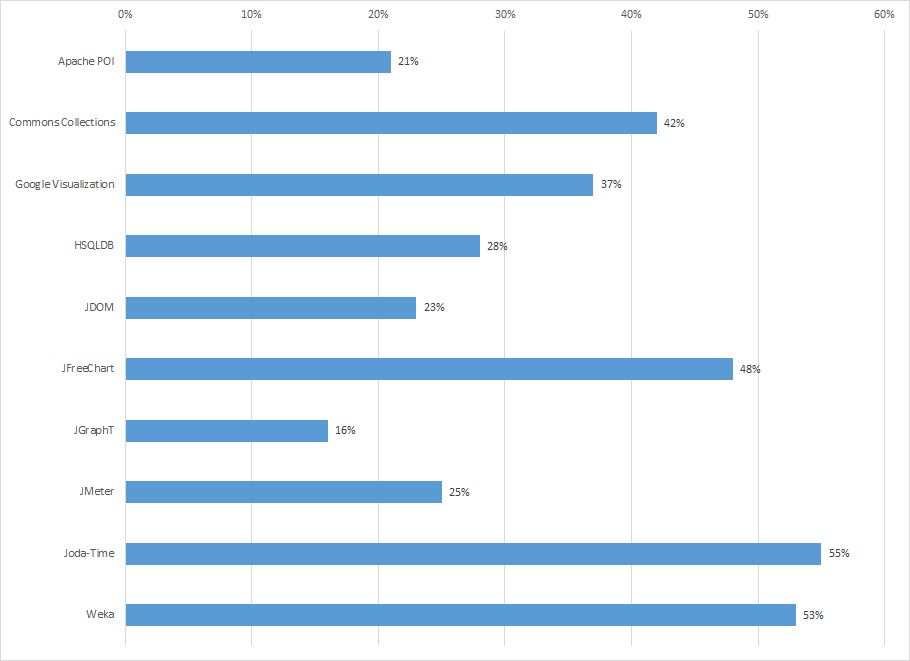
\includegraphics[width=\textwidth, keepaspectratio=true]{images/percent_method_in_set.png}
   }
\end{frame}

\begin{frame}
\frametitle{Results: Asserts vs Methods distribution} {
   \hspace*{0em}
     \begin{figure}
\begin{tikzpicture}
\begin{axis}[
   xlabel={Asserts}, 
   ylabel={Methods},
   scatter src=\thisrow{z},
]
\addplot[
   scatter, 
   only marks, 
   ]
   table
   {data_by_project.dat};
\end{axis}
\end{tikzpicture}
\end{figure}

   }
\end{frame}

\begin{frame}
\frametitle{Results: Sampling, 75\% True Positive rate} {
   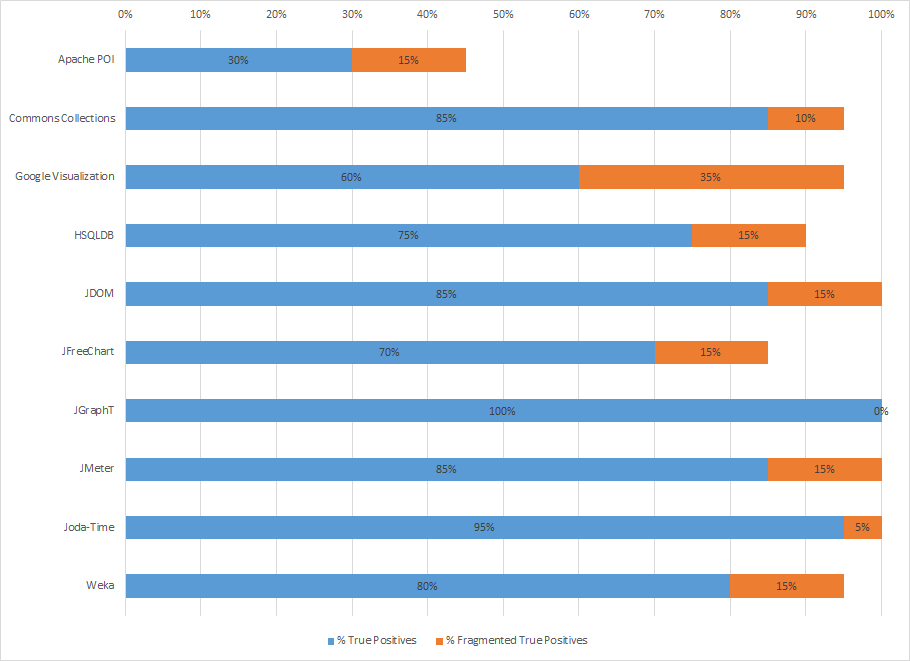
\includegraphics[width=\textwidth, keepaspectratio=true]{images/percent_true_positives.png}
   }
\end{frame}

%% \begin{frame}
%% \frametitle{Results: vs {\tt ccdiml} (Bauhaus), 45\% missed} {
%%    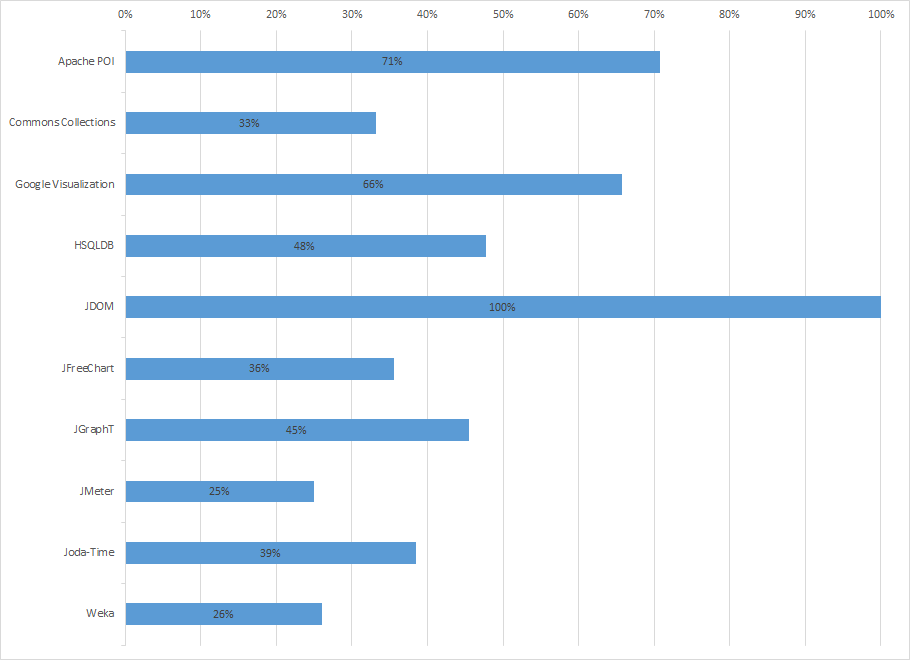
\includegraphics[width=\textwidth, keepaspectratio=true]{images/percent_not_ccdiml.png}
%%    }
%% \end{frame}

\begin{frame}
\frametitle{Qualitative Analysis: JGraphT} {
   \Large
     \begin{itemize}
        \item Small and heterogenous tests that are unlikely to be false positives
     \end{itemize}
}
\end{frame}

\begin{frame}
\frametitle{Qualitative Analysis: Joda-Time} {
   \Large
     \begin{itemize}
        \item Wide hierarchy of tests with identical structures and straight-line assertions.
     \end{itemize}
}
\end{frame}

\begin{frame}
\frametitle{Qualitative Analysis: Weka, Apache Commons Collections} {
   \Large
   \begin{itemize}
      \item Textually identical clones of methods with similar data types
         but with different environment setups.
   \end{itemize}    
}
\end{frame}

\begin{frame}[fragile]
\frametitle{Qualitative Analysis: JDOM} {
\begin{lstlisting}
public void test_TCC___String() {
  // [... 4x assertTrue(String, boolean)]
  try {
    // ...
    fail("allowed creation of an element with no name");
  } catch (IllegalNameException e) { 
    // Test passed!
  }
}
\end{lstlisting}
}
\end{frame}

\begin{frame}
\frametitle{Qualitative Analysis: Google Visualization} {
   \Large
   \begin{itemize}
      \item Complex query-related statements and helper methods reduce
         the roles of assertions in a test method, 
         resulting in a below-average true positive rate.
   \end{itemize}    
}
\end{frame}

\begin{frame}
\frametitle{Qualitative Analysis: Refactorability} {
   \Large
   \begin{itemize}
      \item Test methods that show structural similarities are most likely amenable to
         refatoring, however;
         \vspace{0.5cm}
      \item Non-parametrized and small methods are diffcult to refactor.
   \end{itemize}    
}
\end{frame}

\begin{frame}
  \frametitle{Next Step}

\begin{center}
\Large
Guided test refactoring.
\end{center}
\end{frame}


\section{Future Perspectives}

\begin{frame}
  \frametitle{What Do We Do With Tests?}
\begin{changemargin}{1cm}
\Large
Tradtionally: \\
\hspace*{1em} run the test, get yes/no answer.\\[1em]

(Also, can combine with DSD/concolic analysis.)
\end{changemargin}
\end{frame}

\begin{frame}
  \frametitle{Our usual interaction with tests (static)}

\begin{center}
\begin{tikzpicture}
      \node[draw] (code) { Program };
      \node[draw,left of=code,xshift=-2em,color=gray!80] (test) { Tests };
      \node[draw,below of=code] (tool) { Analysis Tool };
      \node[draw,below of=tool] (gentest) { Generated Tests };

      \path[->,color=gray,dotted] (test) edge[thick] (code);
      \path[->] (code) edge[thick] (tool);
      \path[->] (tool) edge[thick] (gentest);
\end{tikzpicture}
\Large
~\\[1em]
Statically, we usually just ignore tests.
\end{center}
%\Large
%\begin{changemargin}{1cm}
%Test Generation:

%Write-only. Output from static analysis.
%\end{changemargin}
\end{frame}

\begin{frame}
  \frametitle{Our usual interaction with tests (dynamic)}

\begin{center}
\begin{tikzpicture}
      \node[draw] (code) { Program };
      \node[draw,above of=code] (test) { Tests };
      \node[draw,below of=code] (tool) { Analysis Tool };
      \node[draw,below of=tool] (gentest) { Generated Tests };

      \path[->] (test) edge[thick] (code);
      \path[->] (code) edge[thick] (tool);
      \path[->] (tool) edge[thick] (gentest);
\end{tikzpicture}
\Large
~\\[1em]
Tests are write-only with respect to the tool.
\end{center}
%\Large
%\begin{changemargin}{1cm}
%Test Generation:

%Write-only. Output from static analysis.
%\end{changemargin}
\end{frame}

\begin{frame}
  \frametitle{A Better Way}

\begin{center}
\begin{tikzpicture}
      \node[draw] (code) { Program };
      \node[draw,left of=code,xshift=-2em] (test) { Tests };
      \node[draw,below of=code] (tool) { Analysis Tool };
      \node[draw,below of=tool] (gentest) { Generated Tests };

      \path[->] (test) edge[thick] (code);
      \draw[thick, ->] (test) |-  (tool);
      \path[->] (code) edge[thick] (tool);
      \path[->] (tool) edge[thick] (gentest);
\end{tikzpicture}
\Large
\end{center}
\end{frame}

\begin{frame}
  \frametitle{Why is it hard to write tests?}

\begin{changemargin}{1cm}
\Large

Need to:
\begin{enumerate}
\item get system under test in appropriate state;
\item decide what the right answer is.
\end{enumerate}
~\\

Useful hints for static analysis!
\end{changemargin}
\end{frame}

\begin{frame}
  \frametitle{Unit tests also illustrate\ldots}

\begin{changemargin}{1cm}
\Large
\begin{itemize}
\item interesting points in execution space, with
\item complete execution environments \\ \hspace*{2em} for program fragments.
\end{itemize}
\end{changemargin}
\end{frame}

\begin{frame}
  \frametitle{Challenges}

\begin{changemargin}{1cm}
\Large
How to combine information from test runs? \\[1em]
What can we learn from failing tests?
\end{changemargin}
\end{frame}

\section{Conclusions}


\begin{frame}
  \frametitle{Tests: An Opportunity for Program Analysis}
\begin{center}
\Large
We can go beyond test generation.\\[1em]
Tests are a valuable source of information\\ about their associated programs.
\end{center}
\end{frame}

\end{document}
